\documentclass[xetex,mathsans,sans,aspectratio=169]{beamer}
\usepackage{listings}
\usetheme{Boadilla}
\usecolortheme{orchid}
\usepackage{fontspec}
\setsansfont{Basis Grotesque}
\setbeamertemplate{navigation symbols}{}
\usepackage{amsmath}
\usepackage{multicol}


\title[NuCypher]{NuCypher}
\author[Michael]{Michael Egorov, CTO of NuCypher}
\date[28 June 2018]{Big blockchain is watching you, 28 June 2018}

\begin{document}
    \begin{frame}
        \titlepage
        \begin{figure}
            \centering
            
\includegraphics[width=5cm]{pdf/nucypher_logo.pdf}
        \end{figure}
    \end{frame}

    \begin{frame}
        \frametitle{Why}
        \framesubtitle{Encrypted file sharing}
        \begin{figure}
            \centering
            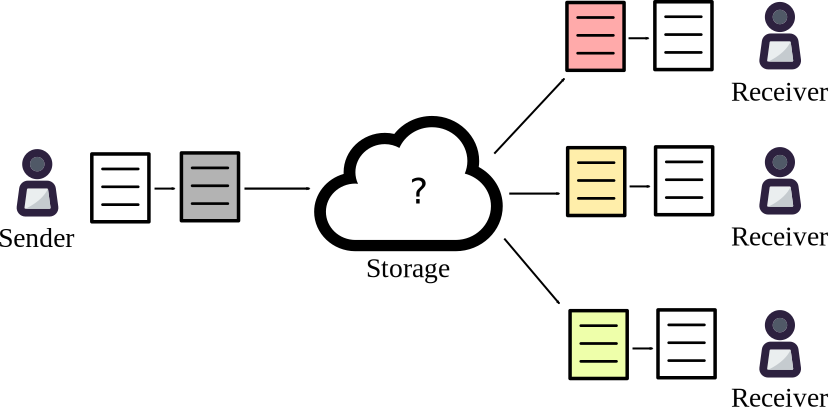
\includegraphics[height=5.5cm]{pdf/file-sharing.pdf}
        \end{figure}
    \end{frame}

    \begin{frame}
        \frametitle{Why}
        \framesubtitle{Encrypted multi-user chats}
        \begin{figure}
            \centering
            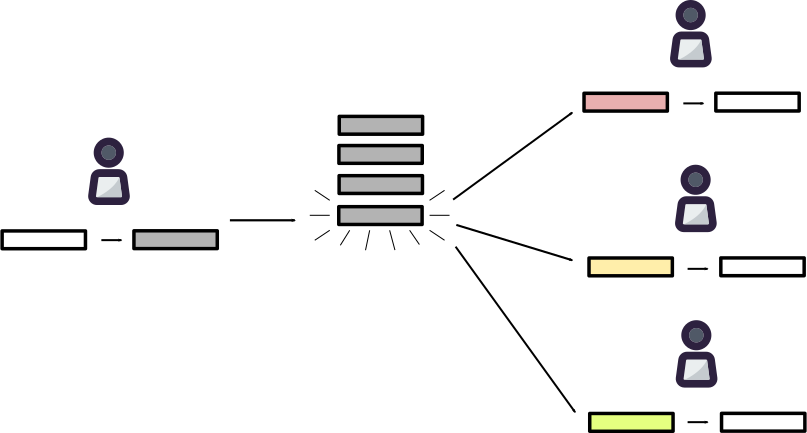
\includegraphics[height=5.5cm]{pdf/chats.pdf}
        \end{figure}
    \end{frame}

    \begin{frame}
        \frametitle{Why}
        \framesubtitle{Decentralized Netflix}
        \begin{figure}
            \centering
            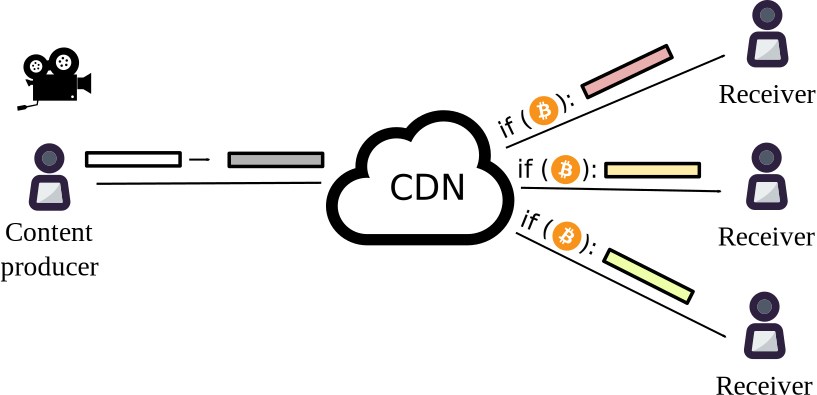
\includegraphics[height=5.5cm]{pdf/streams.pdf}
        \end{figure}
    \end{frame}

    \begin{frame}
        \frametitle{Central server + TLS}
        \framesubtitle{Data vulnerable to hackers, state actors etc}
        \begin{figure}
            \centering
            \includegraphics[width=11cm]{pdf/file-sharing-tls.pdf}
        \end{figure}
    \end{frame}

    \begin{frame}
        \frametitle{Solution}
        \framesubtitle{Proxy re-encryption + decentralization}
        \begin{figure}
            \centering
            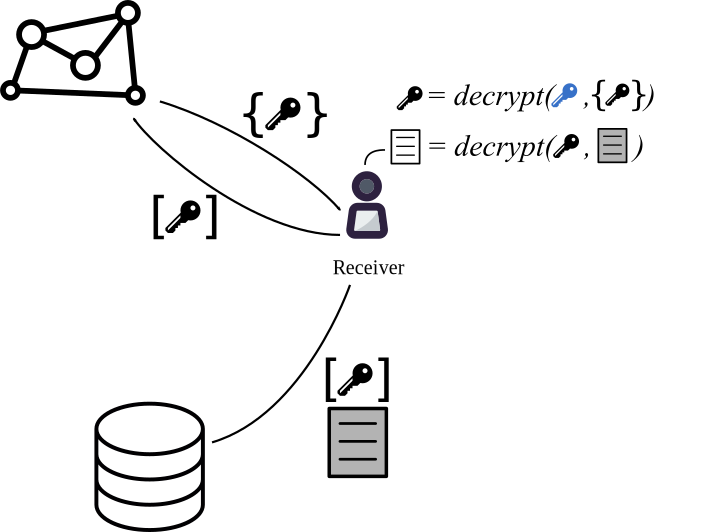
\includegraphics[height=5.5cm]{pdf/pre-kms.pdf}
        \end{figure}
    \end{frame}

    \begin{frame}
        \frametitle{What is proxy re-encryption (PRE)}
        \begin{figure}
            \centering
            \includegraphics[width=11cm]{pdf/pre.pdf}
        \end{figure}
    \end{frame}

    \begin{frame}
        \frametitle{Centralized KMS using PRE}
        \framesubtitle{Encryption}
        \begin{figure}
            \centering
            \includegraphics[height=5.5cm]{pdf/encrypt.pdf}
        \end{figure}
    \end{frame}

    \begin{frame}
        \frametitle{Centralized KMS using PRE}
        \framesubtitle{Access delegation}
        \begin{figure}
            \centering
            \includegraphics[height=5.5cm]{pdf/delegate.pdf}
        \end{figure}
    \end{frame}

    \begin{frame}
        \frametitle{Centralized KMS using PRE}
        \framesubtitle{Decryption}
        \begin{figure}
            \centering
            \includegraphics[height=5.5cm]{pdf/decrypt.pdf}
        \end{figure}
    \end{frame}

    \begin{frame}
        \frametitle{Decentralized key management}
        \framesubtitle{Using threshold split-key re-encryption (Umbral)}
        \begin{figure}
            \centering
            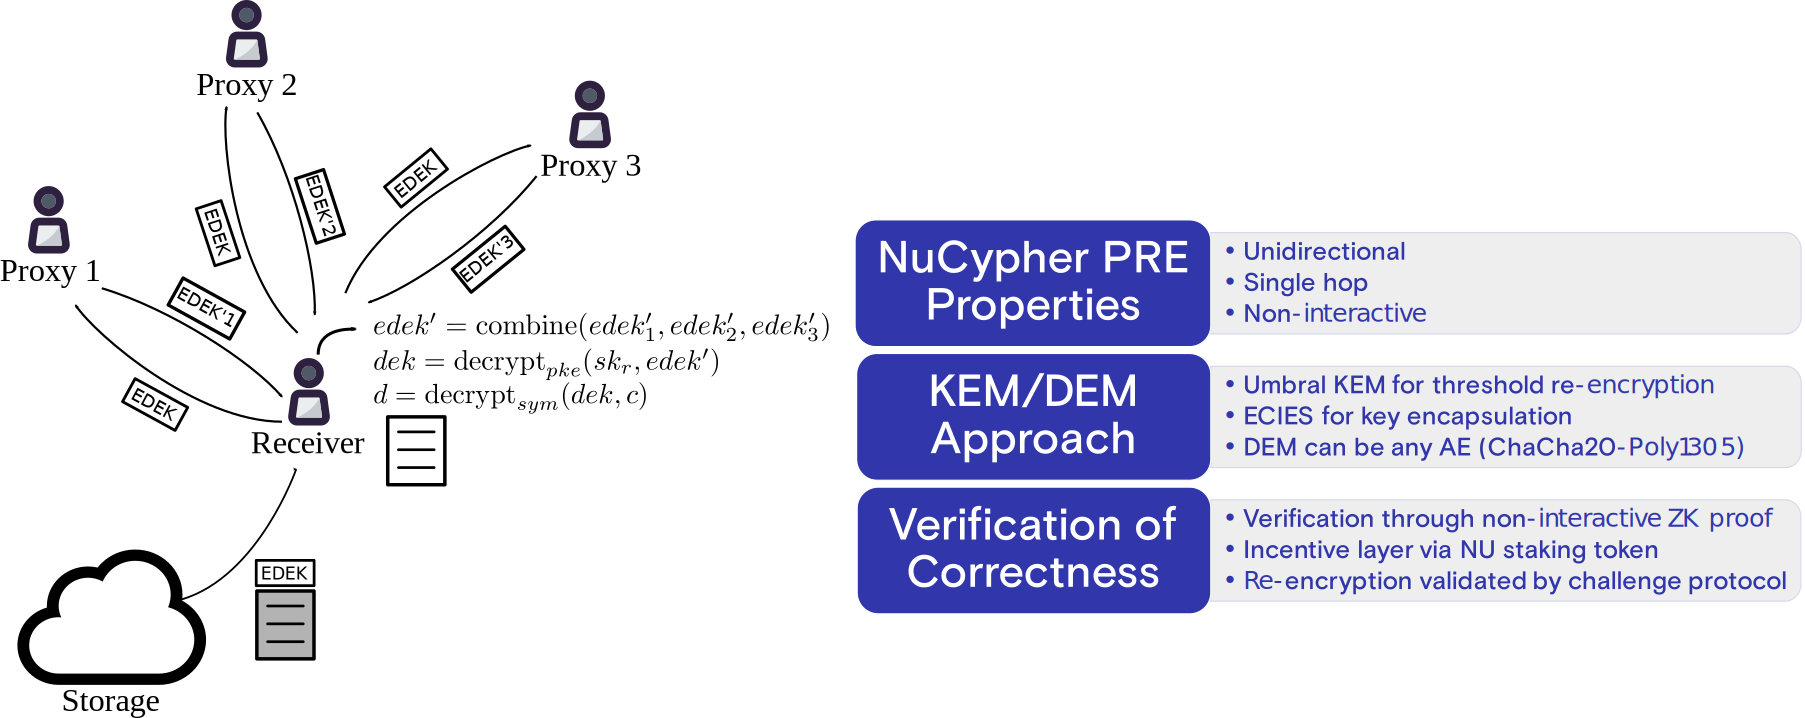
\includegraphics[height=6.5cm]{pdf/decrypt-umbral.pdf}
        \end{figure}
        \url{https://github.com/nucypher/nucypher/}
        \url{https://github.com/nucypher/pyUmbral/}
    \end{frame}

    \begin{frame}
        \frametitle{Umbral: threshold proxy re-encryption}
        %\framesubtitle{Purpose}
        \begin{itemize}
        	\item \emph{``Umbral''} is Spanish for \emph{``threshold''}
            \item PRE properties: Unidirectional, single-hop, non-interactive
            \item It follows a KEM/DEM approach:
            	\begin{itemize}
					\item UmbralKEM provides the threshold re-encryption capability
                    \item Encryption is ECIES with extra things for proof of correctness, on curve \emph{secp256k1}
            		\item The DEM can be any authenticated encryption (currently ChaCha20-Poly1305)
        		\end{itemize}
			\item IND-PRE-CCA security
			\item Verification of re-encryption correctness through Non-Interactive ZK Proofs
			\item Code: \url{https://github.com/nucypher/pyUmbral/}
			\item Documentation (WIP): \url{https://github.com/nucypher/umbral-doc}
        \end{itemize}
    \end{frame}

    \begin{frame}
        \frametitle{PRE demo}
        \begin{figure}
            \centering
            \includegraphics[height=5.5cm]{pdf/terminal.pdf}
        \end{figure}
        Demo network: \url{https://github.com/nucypher/mock-net/}
    \end{frame}

    \begin{frame}
        \frametitle{NU token}
        \framesubtitle{Purpose}
        \begin{itemize}
            \item Splitting trust between re-encryption nodes (more tokens = more trust and more work);
            \item Proof of Stake for minting new coins according to the mining schedule;
            \item Security deposit to be at stake against malicious behavior of nodes
        \end{itemize}
    \end{frame}

    \begin{frame}
        \frametitle{NU token}
        \framesubtitle{Mining}
        Mining reward:
        \begin{eqnarray}
            \kappa &=& \left(0.5 + 0.5\frac{\min(T_i, T_1)}{T_1}\right)\\
            T_{i,\text{initial}} &\ge& T_{\min},\\
            \delta s_{i,t} &=&  \kappa\, \frac{l_i}{\sum l_j} \frac{\ln{2}}{T_{1/2}} \left( S_{\max} - S_{t-1}\right).\\
        \end{eqnarray}
        Results into:
        $$\text{reward} \propto 2^{\frac{t}{T_{1/2}}}$$
    \end{frame}

    \begin{frame}
        \frametitle{NU token}
        \framesubtitle{Graph of daily mining compensation}
        \begin{equation}
            \text{reward}_i = \kappa_i \cdot \text{reward}_0,\qquad
            \kappa^* = \left< \kappa_i \right>,\qquad
            \lambda = \frac{S_{\text{locked}}}{S};
        \end{equation}
        \begin{equation}
            T_{1/2}^* = T_{1/2} / \kappa^*.
        \end{equation}
        \begin{figure}
            \centering
            \includegraphics[height=5.5cm]{pdf/daily-compensation.pdf}
        \end{figure}
    \end{frame}

    \begin{frame}
        \frametitle{NU token}
        \framesubtitle{Relocking mining rewards}
        \small{
        \begin{equation}
            \frac{c_{\text{dump}}}{\text{stake}} =
            \frac{\kappa}{\kappa^* \lambda} \ln \frac{S(t)}{S_0};
        \end{equation}
        \begin{equation}
            \frac{c_{\text{hodl}}}{\text{stake}} =
            \left[ \frac{S(t)}{S_0} \right] ^ {\frac{\kappa}{\kappa^* \lambda}};
        \end{equation}}
        \begin{figure}
            \centering
            \includegraphics[height=5.5cm]{pdf/total-compensation.pdf}
        \end{figure}
    \end{frame}

    \begin{frame}
        \frametitle{Usage examples}
        \begin{multicols}{2}
            Decentralized marketplaces:
            \begin{itemize}
                \item Datum;
                \item Origin protocol;
                \item The Seam;
                \item SwipeCrypto.
            \end{itemize}
            Decentralized databases:
            \begin{itemize}
                \item Bluzelle;
                \item Fluence;
                \item Wolk.
            \end{itemize}
            Medical data sharing
            \begin{itemize}
                \item Medibloc;
                \item IRYO;
                \item Medixain;
                \item Wholesome;
                \item Medcredits;
                \item HealthCombix / PointNurse;
                \item Genobank;
                \item iku.network.
            \end{itemize}
            IoT
            \begin{itemize}
                \item Spherity (together with BigchainDB);
                \item Carblock.io;
                \item XAIN.
            \end{itemize}
            Cryptocurrency keys
            \begin{itemize}
                \item Coval Emblem Vault.
            \end{itemize}
        \end{multicols}
    \end{frame}

    \begin{frame}
        \frametitle{Useful links}
        \begin{figure}
            \centering
            
\includegraphics[width=5cm]{pdf/nucypher_logo.pdf}
        \end{figure}
        Website: \url{https://nucypher.com}

        Github: \url{https://github.com/nucypher/}

        PyUmbral on Github: \url{https://github.com/nucypher/pyUmbral/}

        Mochnet: \url{https://github.com/nucypher/mock-net/}

        Discord: \url{https://discord.gg/7rmXa3S}

        Whitepaper: \url{https://arxiv.org/abs/1707.06140}

        E-mail: \url{michael@nucypher.com}

        E-mail: \url{hello@nucypher.com}
    \end{frame}

\end{document}

